%%%%%%%%%%%%%%%%%%%%%%%%%%%%%%%%%%%%%%%%%
% Beamer Presentation
% LaTeX Template
% Version 1.0 (10/11/12)
%
% This template has been downloaded from:
% http://www.LaTeXTemplates.com
%
% License:
% CC BY-NC-SA 3.0 (http://creativecommons.org/licenses/by-nc-sa/3.0/)
%
%%%%%%%%%%%%%%%%%%%%%%%%%%%%%%%%%%%%%%%%%

%----------------------------------------------------------------------------------------
%	PACKAGES AND THEMES
%----------------------------------------------------------------------------------------

\documentclass{beamer}



\mode<presentation> {



% The Beamer class comes with a number of default slide themes
% which change the colors and layouts of slides. Below this is a list
% of all the themes, uncomment each in turn to see what they look like.

%\usetheme{default}
%\usetheme{AnnArbor}
%\usetheme{Antibes}
%\usetheme{Bergen}
%\usetheme{Berkeley}
%\usetheme{Berlin}
%\usetheme{Boadilla}
%\usetheme{CambridgeUS}
%\usetheme{Copenhagen}
%\usetheme{Darmstadt}
%\usetheme{Dresden}
%\usetheme{Frankfurt}
%\usetheme{Goettingen}
%\usetheme{Hannover}
%\usetheme{Ilmenau}
%\usetheme{JuanLesPins}
%\usetheme{Luebeck}
%\usetheme{Madrid}
%\usetheme{Malmoe}
%\usetheme{Marburg}
%\usetheme{Montpellier}
%\usetheme{PaloAlto}
%\usetheme{Pittsburgh}
%\usetheme{Rochester}
%\usetheme{Singapore}
%\usetheme{Szeged}
%\usetheme{Warsaw}

% As well as themes, the Beamer class has a number of color themes
% for any slide theme. Uncomment each of these in turn to see how it
% changes the colors of your current slide theme.

%\usecolortheme{albatross}
%\usecolortheme{beaver}
%\usecolortheme{beetle}
%\usecolortheme{crane}
%\usecolortheme{dolphin}
%\usecolortheme{dove}
%\usecolortheme{fly}
%\usecolortheme{lily}
%\usecolortheme{orchid}
%\usecolortheme{rose}
%\usecolortheme{seagull}
%\usecolortheme{seahorse}
%\usecolortheme{whale}
%\usecolortheme{wolverine}

%\setbeamertemplate{footline} % To remove the footer line in all slides uncomment this line
%\setbeamertemplate{footline}[page number] % To replace the footer line in all slides with a simple slide count uncomment this line

%\setbeamertemplate{navigation symbols}{} % To remove the navigation symbols from the bottom of all slides uncomment this line




\usepackage{siunitx}
\usetheme{Madrid}
\useoutertheme{miniframes} % Alternatively: miniframes, infolines, split
\useinnertheme{circles}
\beamertemplatenavigationsymbolsempty

%\definecolor{UBCblue}{rgb}{0.04706, 0.13725, 0.26667} % UBC Blue (primary)
%\definecolor{UBCgrey}{rgb}{0.3686, 0.5255, 0.6235} % UBC Grey (secondary)
%%\definecolor{crcgreen}{rgb}{116/255, 198/255, 155/255}
%\definecolor{crcgreen}{rgb}{0.454, 0.776, 0.608}
%\setbeamercolor{palette primary}{bg=white,fg=crcgreen}
%\setbeamercolor{palette secondary}{bg=white,fg=white}
%\setbeamercolor{palette tertiary}{bg=white,fg=white}
%\setbeamercolor{palette quaternary}{bg=white,fg=white}
%\setbeamercolor{structure}{fg=white} % itemize, enumerate, etc
%\setbeamercolor{section in toc}{fg=white} % TOC sections
%
%% Override palette coloring with secondary
%\setbeamercolor{subsection in head/foot}{bg=white,fg=white}






}

\date{12th International Conference on Urban Climate (ICUC12), Rotterdam, The Netherlands, 7–11 Jul 2025}
\usepackage{bibentry}
\nobibliography*
\usepackage{multicol}
%\usepackage{ulem}
\usepackage{graphicx} % Allows including images
%\usepackage{booktabs} % Allows the use of \toprule, \midrule and \bottomrule in tables
\usepackage[sort&compress,square,comma,authoryear]{natbib}
\bibliographystyle{plainnat}
%\bibliographystyle{kerry_harvard}
\renewcommand\bibfont{\scriptsize}

 \newcommand\makebeamertitle{\frame{\maketitle}}%
 
 \beamertemplatenavigationsymbolsempty
 \setbeamertemplate{headline}{}

%----------------------------------------------------------------------------------------
%	TITLE PAGE
%----------------------------------------------------------------------------------------



\begin{document}


\title[The SIMPEL soil water balance module]{Improving urban water process representations in land surface models with the SIMPEL soil water balance module}
\author[Nice, KA et al.]
{Kerry A. Nice$^{1}$, Harro J. Jongen$^{2}$, Kristian Förster$^{3}$
}
\institute[UoM]{{\begin{flushleft}
\tiny $^{1}$ Transport, Health, and Urban Systems Research Lab, Faculty of Architecture, Building and Planning, University of Melbourne.\\$^{2}$ Institute for Water and Environment, Karlsruhe Institute of Technology, Karlsruhe, Germany.\\$^{3}$ Institute of Ecology and Landscape, Department of Landscape Architecture, Hochschule Weihenstephan-Triesdorf, Freising, Germany.
\end{flushleft}}}
\titlegraphic{
\includegraphics[scale=0.75]{template_icuc12_logo.png}~~~~
\includegraphics[scale=0.5]{image001.jpg}~~~
\includegraphics[scale=0.10]{karlsruhe-institute-of-technology-kit-logo-png_seeklogo-353008_.png}~~~
\includegraphics[scale=0.12]{Hochschule_Weihenstephan-Triesdorf_Logo.svg.png}}
\makebeamertitle


%


\begin{frame}{Motivation: Modelling irrigation} 

\begin{itemize}
\item Irrigation trials at University of Melbourne (Burnley)$^{1}$. Looking for model capable of reproducing micro-scaled results.\\ 
\item But most hydrology models are at a catchment scale.
\end{itemize}
\begin{center}
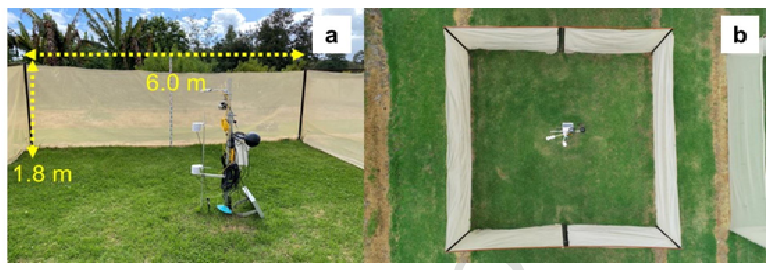
\includegraphics[scale=0.60]{Screenshot_20250703_100546.png}
\end{center}
$^{1}${\footnotesize \cite{Cheung2024}, 10.5281/zenodo.10140668, 10.5281/zenodo.10972538}
\end{frame}






\begin{frame}{Motivation: Urban Plumber} 
\begin{itemize}

\item Meanwhile, Urban Plumber results: most urban models do a terrible job with hydrology {\footnotesize \citep{jongen_water_2024}}.
\begin{itemize}
\item Most don't account for hydrology at all
\item If they do, water budget rarely closed
\item Or fully account for all types of indicators (runoff, infiltration, ET, storage)
\item Leading to less accurate modelling
\end{itemize}
\item Urban Plumber and previous intercomparisions: Latent energy fluxes in urban areas poorly predicted by most models {\footnotesize \citep{lipson_evaluation_2024,grimmond_initial_2011}}
\end{itemize}
\end{frame}









\begin{frame}{The SIMPEL model} 


\begin{columns}

\begin{column}{0.5\textwidth}
\begin{itemize}
\item Single bucket model
\item original Excel spreadsheet developed by Georg Hörmann
\item extended (snow, surface runoff) by Kristian Förster 2022
\item Adapted by Kerry Nice 2023-5
\item Support hourly timesteps, irrigation
\end{itemize}
\end{column}

\begin{column}{0.5\textwidth}
 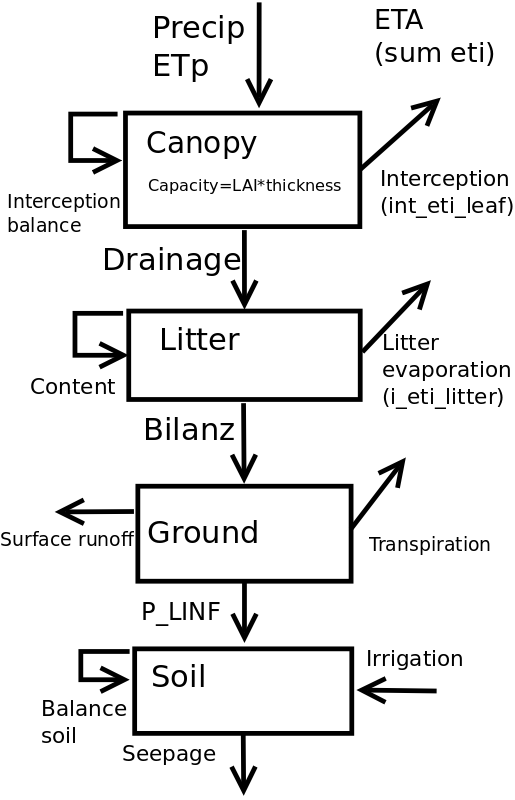
\includegraphics[scale=0.30]{Simpel_diagram2.png}\\
Adapted from \cite{hormann_comparison_2007}
\end{column}

\end{columns}




\end{frame}



\begin{frame}{Validations against Burnley irrigation observations} 
\begin{center}
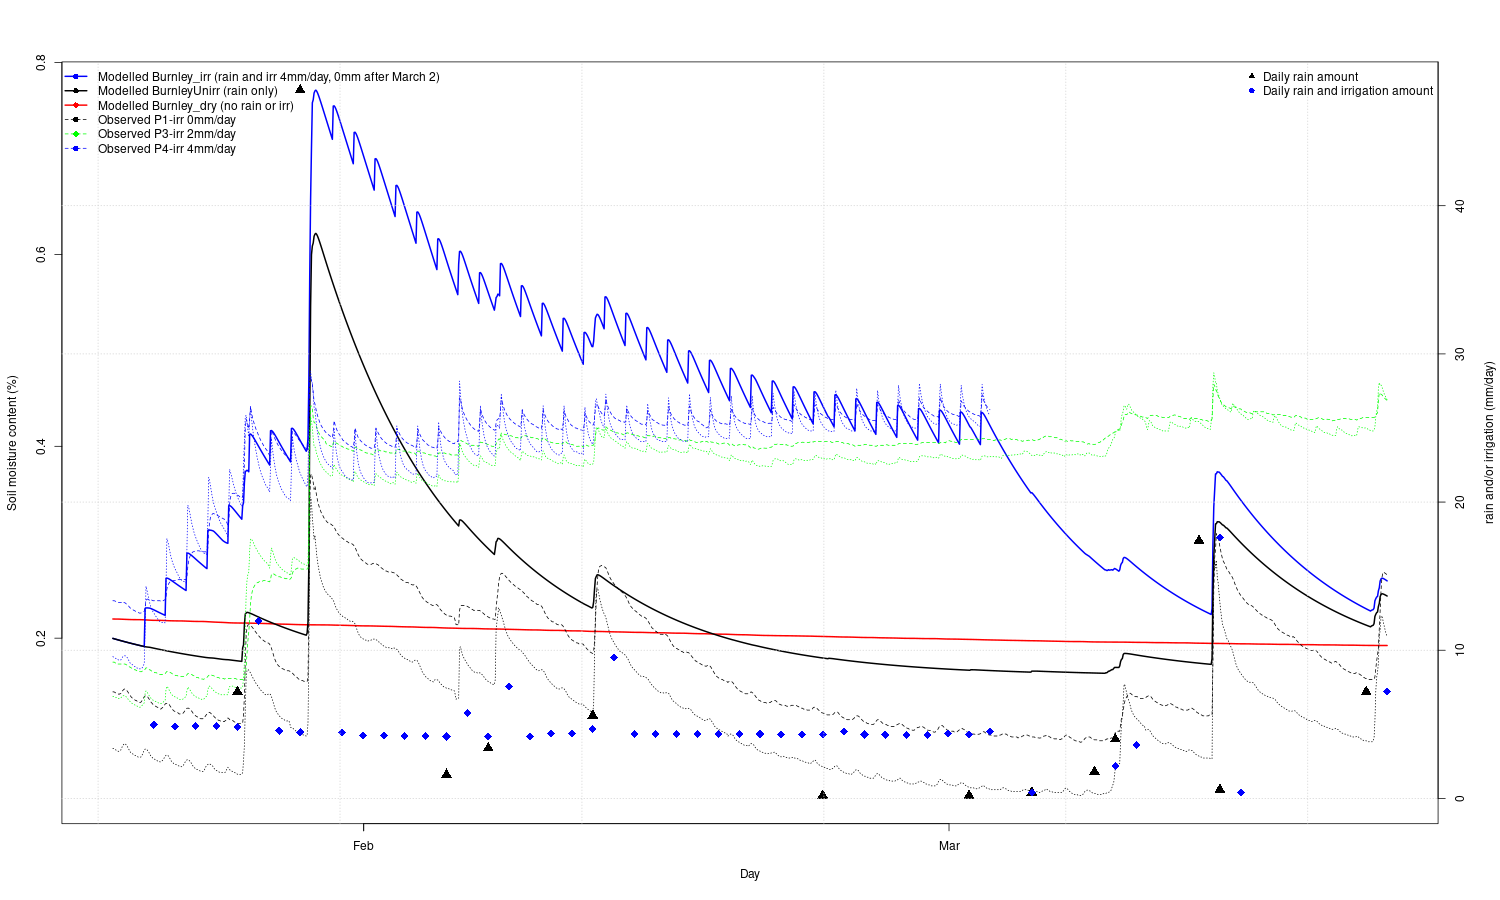
\includegraphics[scale=0.18]{BurnleyComparisons.png}
\end{center}

Initial testing of SIMPEL model with Burnley observations were promising. Reproducing soil moisture of different irrigation amounts (0, 2, 4mm/day).
\\
$^{1}${\footnotesize \cite{Cheung2024}, 10.5281/zenodo.10140668, 10.5281/zenodo.10972538}
\end{frame}



\begin{frame}{The SIMPEL evaporotranspiration comparisons with Urban Plumber sites} 

{\footnotesize And broad agreement across many Urban Plumber sites of evaporotranspiration levels}
\begin{center}
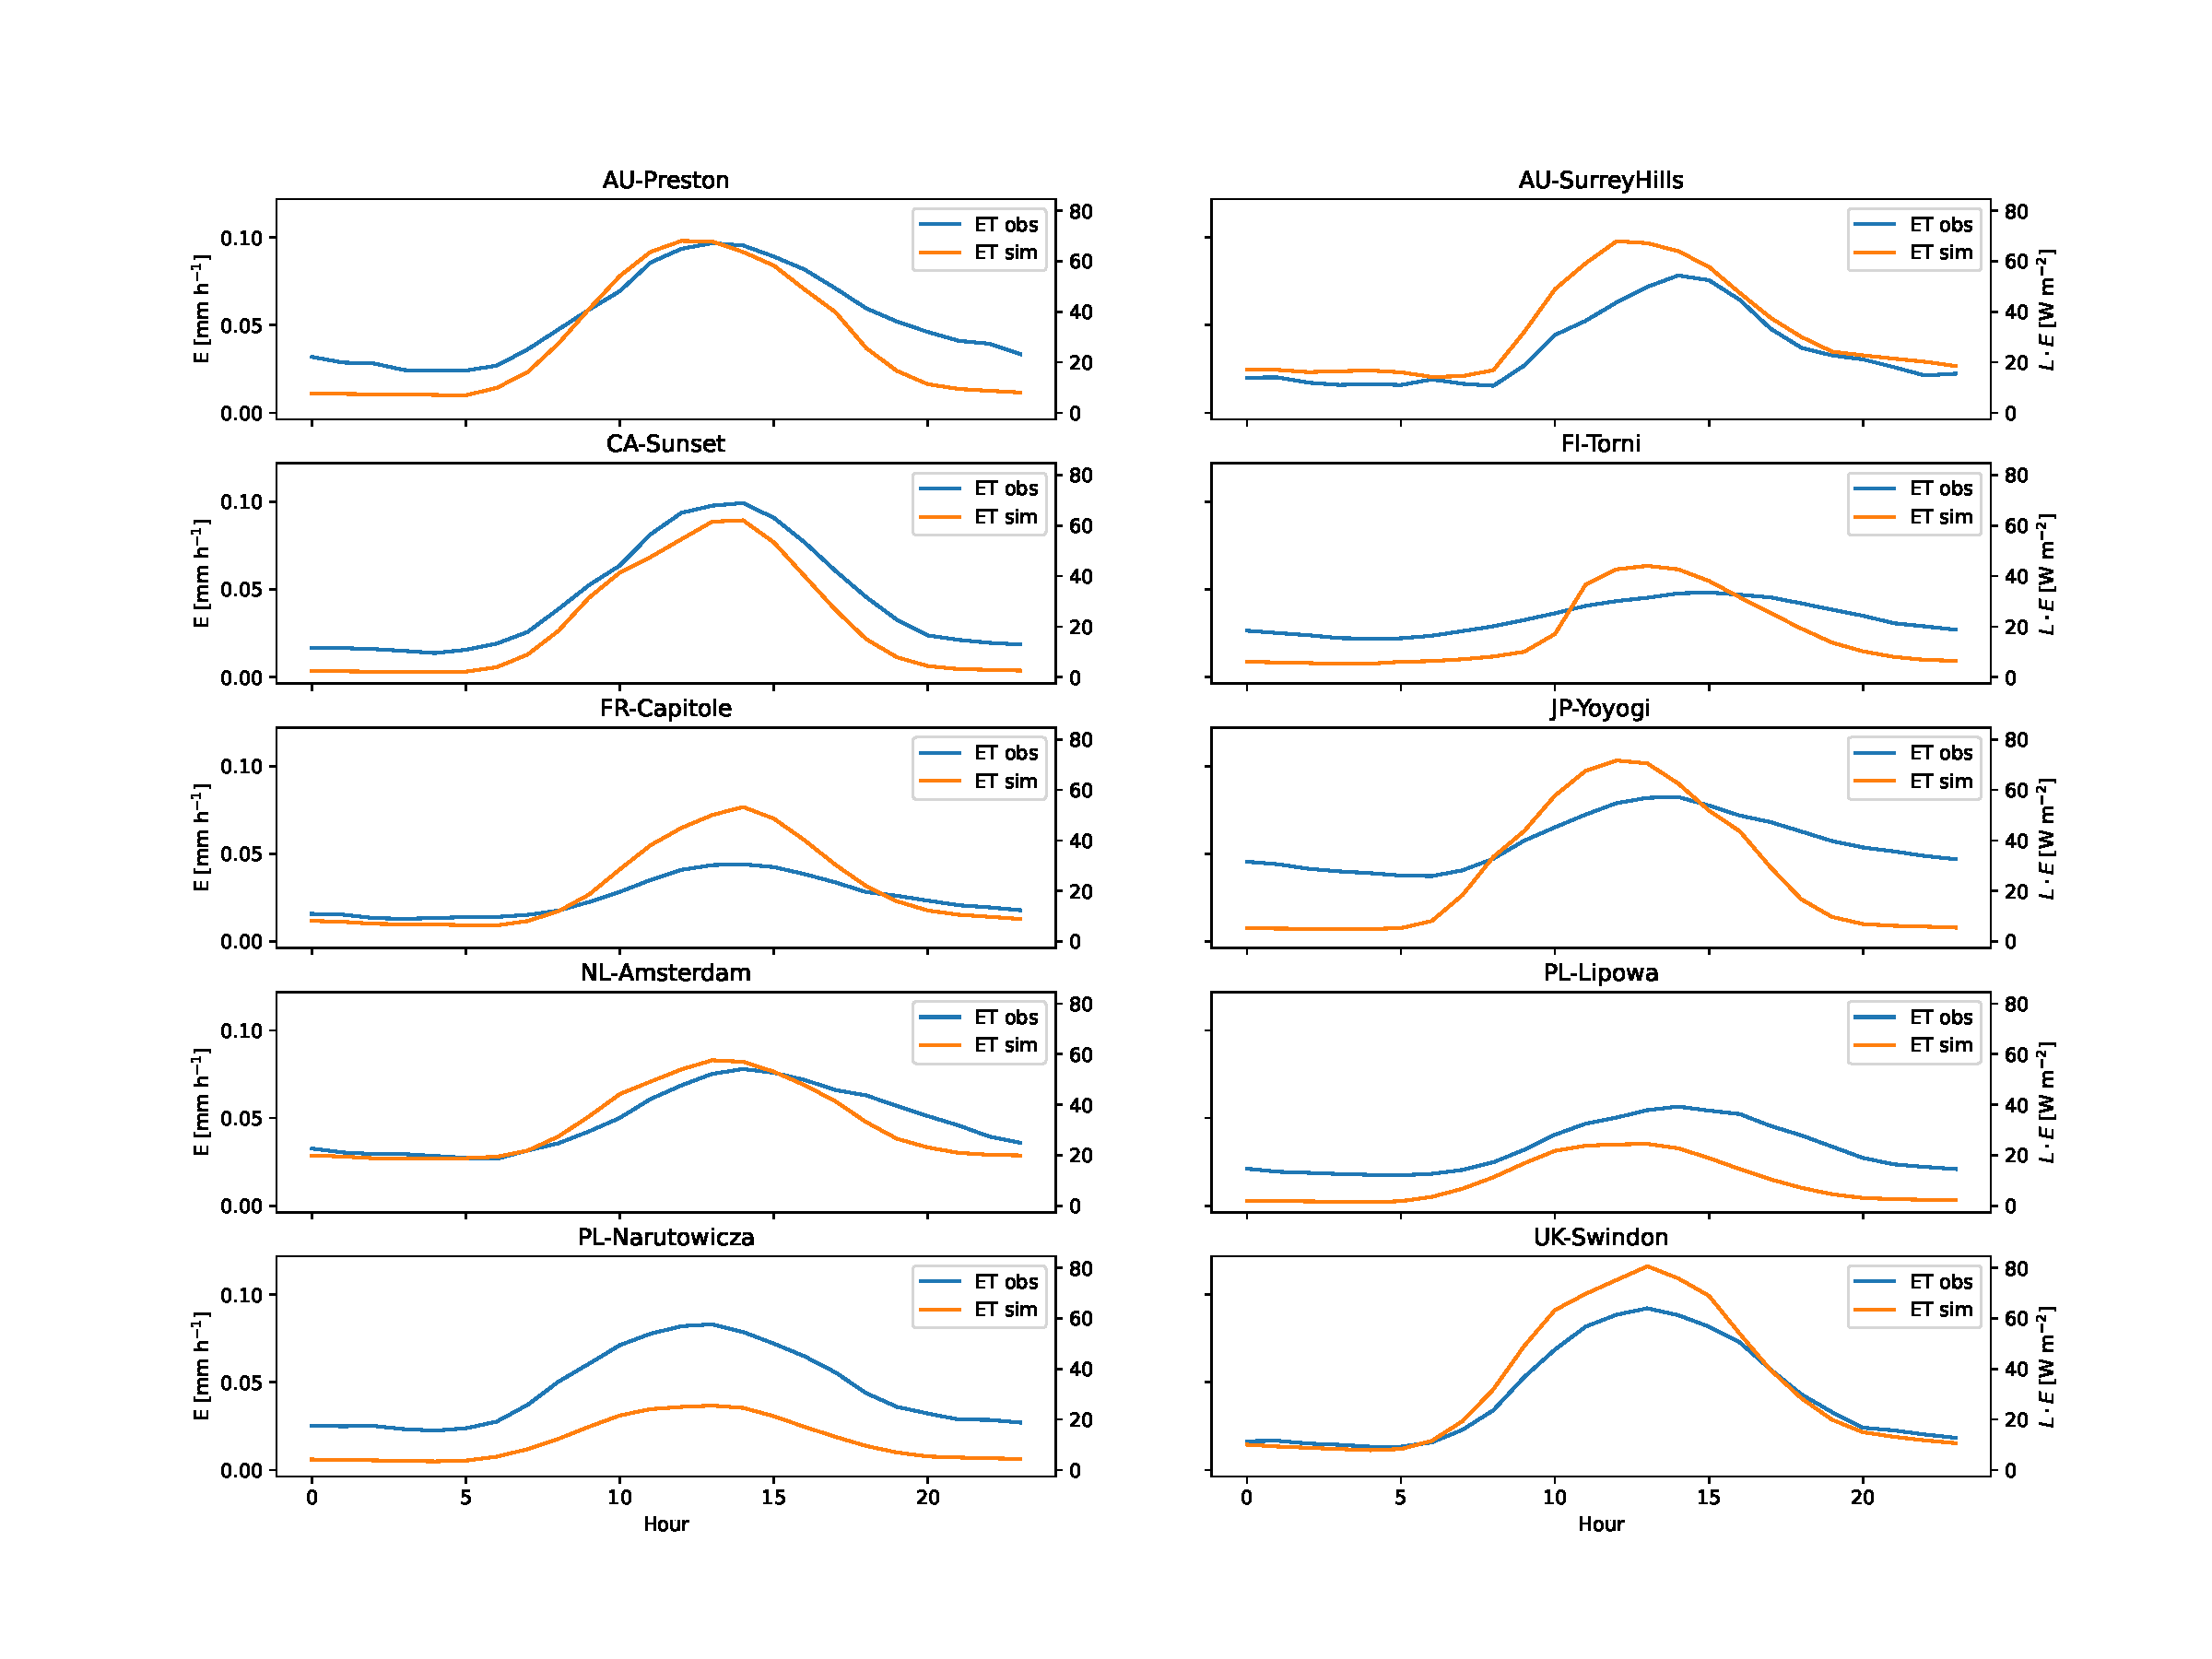
\includegraphics[scale=0.24]{et_presunangle.pdf}
\end{center}
\end{frame}



\begin{frame}{The SIMPEL water balance comparisons with Urban Plumber sites} 
And includes necessary components for water balance closure
\begin{center}
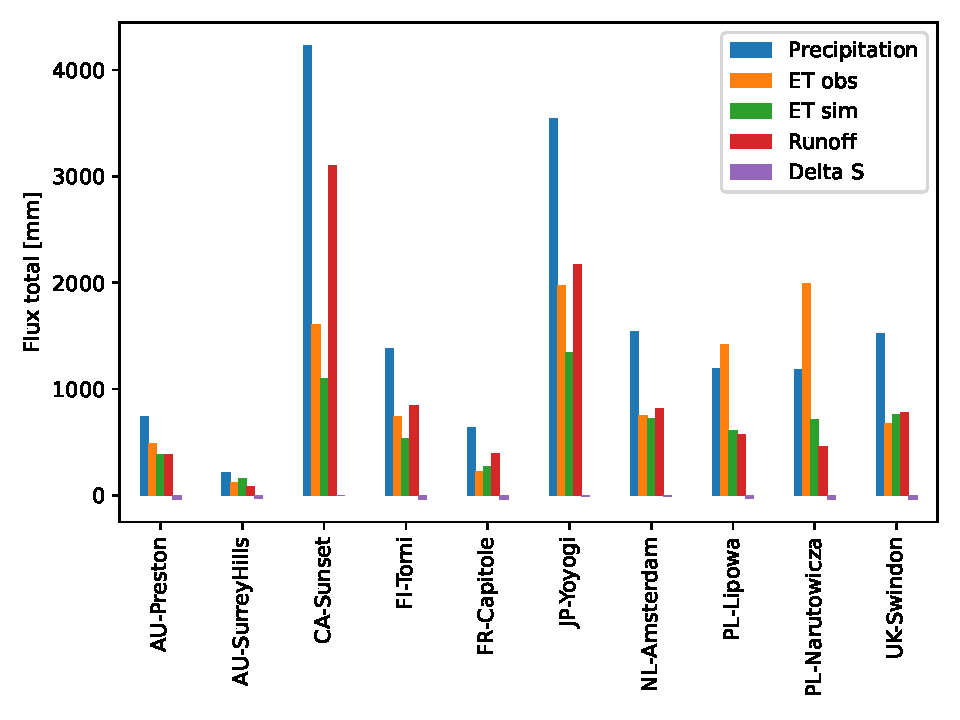
\includegraphics[scale=0.50]{water_balance_presunangle.pdf}
\end{center}
\end{frame}



\begin{frame}{Integration into TARGET} 

\begin{center}
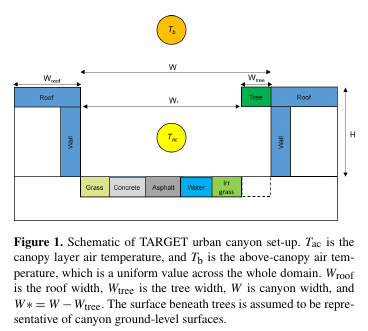
\includegraphics[scale=0.60,trim={20 80 20 10},clip]{TARGET1.png}
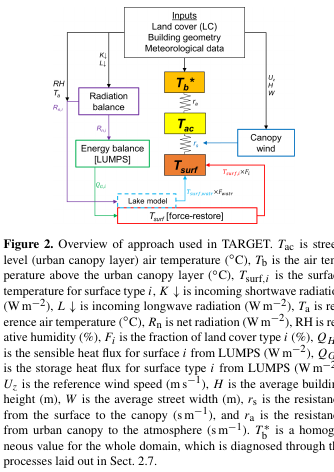
\includegraphics[scale=0.60,trim={20 180 20 0},clip]{TARGET2.png}
\end{center}
The Air-temperature Response to Green/blue-infrastructure Evaluation Tool (TARGET) is a computationally efficient model designed to evaluate blue/green infrastructure, based on an urban canyon and aggregations of different land cover types \citep{Broadbent2019}.
\end{frame}


\begin{frame}{Integration into TARGET} 

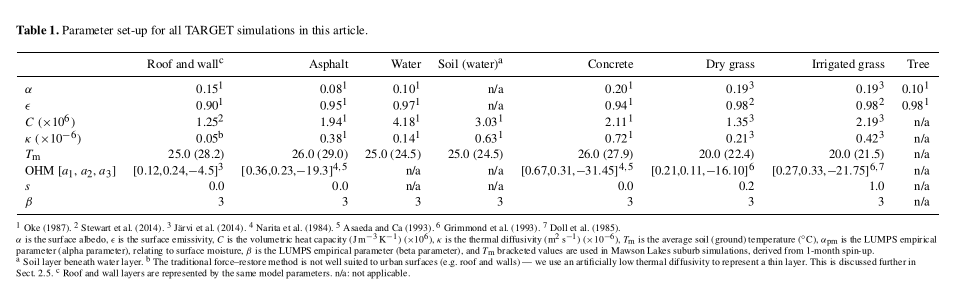
\includegraphics[scale=0.45]{TARGET3.png}

\begin{itemize}
\item Hydrology is not included
\item Latent energy indirectly calculated from ground flux heat storage calculations for different surface types using the $\alpha$ coefficient of the OHM model
\item SIMPLE allows replacement with hydrologically based evaporotranspiration and latent energy calculations.
\item Provides additional capability to account for irrigation, drought and other hydrological impacts
\end{itemize}

\end{frame}


\begin{frame}{Validations against Urban Plumber Preston observations using TARGET} 
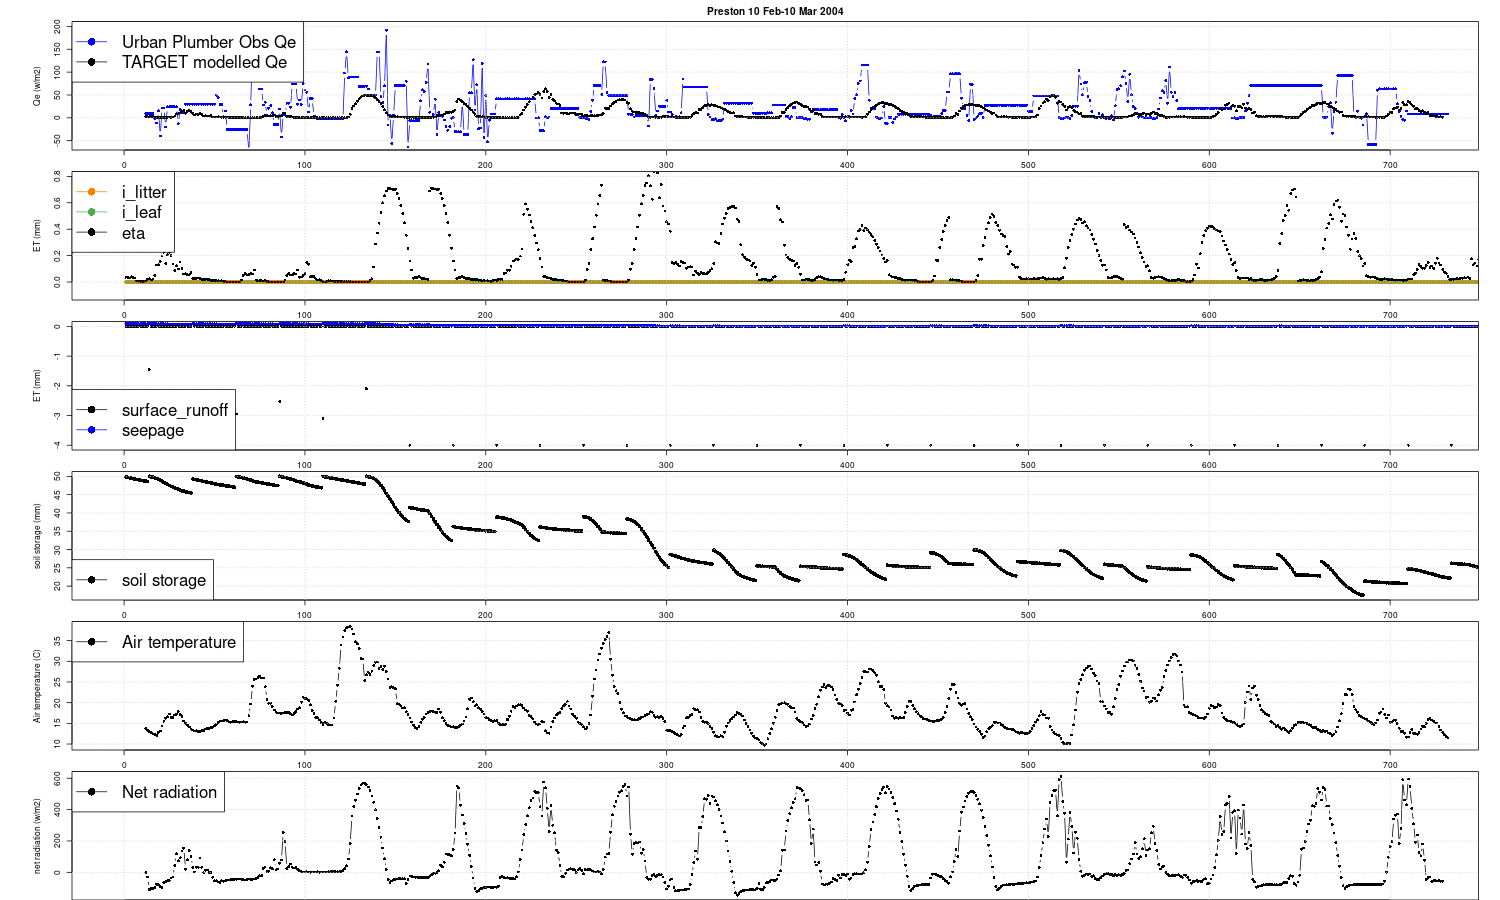
\includegraphics[scale=0.20]{PrestonFeb2004_4mmIrr_ground.png}
\end{frame}


\begin{frame}{Future plans} 

\begin{itemize}

\item Integration into TARGET as a single surface type (irrigated grass) is nearly complete

\item Integration into VTUF-3D as gridded individual buckets for pervious and vegetated surfaces is planned

\item Improvement of ET using stomatal models to incorporate additional vegetation types

\item SIMPEL model could also be integrated into other urban models, providing a micro-scaled hydrology for a variety of vegetated and pervious surface types

\item Or more accurate runoff for impervious surfaces

% target -> UMEP (workshop Thursday)
%https://github.com/mothlight/Simpel
%https://github.com/mothlight/Target-Java.v2
%https://github.com/mothlight/VTUF-3D-Java.v2/
%https://umep-docs.readthedocs.io/en/latest/processor/Urban%20Heat%20Island%20TARGET.html

\end{itemize}


\end{frame}



%\begin{frame}{Overall workflow} 
%\begin{center}
%
%\begin{figure}[ht]
%\centering
%%\includegraphics[page=1,trim={10 60 20 35},clip,scale=0.50]{figures/GraphicalAbstract4.pdf}
% \label{fig:process}
%\end{figure} 
%\end{center}
%
%\scalebox{0.30}{Kerry A. Nice, Negin Nazarian, Mathew J. Lipson, Melissa A. Hart, Sachith Seneviratne, Jason Thompson, Marzie Naserikia, Branislava Godic, and Mark Stevenson, Isolating the impacts of urban form and fabric from geography on urban heat and human thermal comfort, Building and Environment, 2022. }
%\end{frame}


%\begin{frame}{VTUF-3D micro-climate model} 
%\begin{center}
%
%\includegraphics[page=6,trim={50 20 50 130},clip,scale=0.30]{/home/kerryn/git/2018-02-SingaporeCooling/KerrySingaporeCooling.pdf}
%\\
%\includegraphics[page=7,trim={50 40 100 60},clip,scale=0.35]{/home/kerryn/git/2018-02-SingaporeCooling/KerrySingaporeCooling.pdf}
%\\ \scalebox{0.30}{ K.A. Nice, A. Coutts, and N.J. Tapper, Development of the VTUF-3D v1.0 urban micro-climate model to support assessment of urban vegetation influences on human thermal comfort. Urban Climate, 2018. }
%\end{center}
%\end{frame}



%
%
%\begin{frame}{VTUF-3D micro-climate model} 
%\begin{center}
%%\fbox{
%\includegraphics[page=8,trim={50 50 100 130},clip,scale=0.55]{/home/kerryn/git/2018-02-SingaporeCooling/KerrySingaporeCooling.pdf}
%%}
%\end{center}
%\end{frame}
%
%
%
%
%
%
%
%\begin{frame}{Creation of VTUF-3D scenarios for 9814 variations of parameters across representative ranges in Melbourne} 
%\begin{center}
%\begin{figure}
%\centering
%\includegraphics[page=15,trim={70 245 80 240},clip,scale=0.40]{Figures/Figures6.pdf}
%\tiny \\
%Example scenarios from the 9814 modelled 
%\begin{itemize}
%\item 49\% grass, 50\% trees, 0.5\% roads, 0.5\% building, mean building height 5.0m, mean vegetation height 15.0m 
%\item 9\% grass, 0\% trees, 31\% roads, 60\% building, mean building height 49.8m, mean vegetation height 0m
%\item 9\% grass, 10\% trees, 71\% roads, 10\% building, mean building height 14.8m , mean vegetation height 0.5m. 
%\item Modelled 3-dimensional results of UTCI for scenario (c) at 2pm February 12, 2004.
%\end{itemize}
%
%
%\end{figure} 
%\end{center}
%\end{frame}
%
%
%
%\begin{frame}{Forcing data for comparison day} 
%\begin{center}
%\begin{figure}
%\centering
%\includegraphics[page=20,trim={56 288 60 280},clip,scale=0.65]{Figures/Figures6.pdf}
% \label{fig:scenarios}
%\end{figure} 
%\end{center}
%\end{frame}
%
%
%
%
%
%
%
%
%
%
%
%\begin{frame}{Air temperature over surface and height ranges} 
%\begin{center}
%\begin{figure}
%\centering
%\includegraphics[page=2,trim={90 238 90 238},clip,scale=0.55]{Figures/Figures6.pdf}
%\\
%{\tiny Mean $T_{can}$ outcomes clustered by 10\% surface fraction ranges of a) grass, b) streets, c) trees, and d) buildings and e) average vegetation and f) average building heights clustered by 0.8m increases over a diurnal cycle of February 12, 2004\par } 
% \label{fig:tcanday}
%\end{figure}
%\end{center}
%\end{frame}
%
%\begin{frame}{UTCI temperature over surface and height ranges} 
%\begin{center}
%\begin{figure}
%\centering
%\includegraphics[page=3,trim={90 238 90 238},clip,scale=0.55]{Figures/Figures6.pdf}
%\\
%{\tiny  Mean UTCI outcomes clustered by 10\% surface fraction ranges of a) grass, b) streets, c) trees, and d) buildings and e) average vegetation and f) average building heights clustered by 0.8m increases over a diurnal cycle of February 12, 2004.\par } 
% \label{fig:tcanday}
%\end{figure}
%\end{center}
%\end{frame}
%
%
%
%\begin{frame}{Temperature differences summary} 
%\begin{center}
%\begin{figure}
%\centering
%
%\includegraphics[page=10,trim={120 640 120 130},clip,scale=0.8]{/home/unimelb.edu.au/knice/git/2020-07-Frontiers-UrbClimInformatics/Article/MCZArticleV2_Preprint_R1.pdf}
%\\~\\
%Maximum differences ($^{\circ}$C) in T$_{can}$ and UTCI when increasing fractions from 10\% to 90\% and average vegetation and building heights to 4.4m. Bold indicates temperatures increase as fractions or heights increase. 
%\end{figure} 
%\end{center}
%\end{frame}
%
%
%
%
%
%
%
%
%
%\begin{frame}{} 
%\begin{center}
%\begin{figure}
%\centering
%%\includegraphics[page=1,trim={80 90 80 90},clip,scale=0.30]{Figures/Figures6.pdf}
%%\includegraphics[page=1,trim={80 90 80 90},clip,scale=0.30]{Figures/Figures6.pdf}
%%\includegraphics[trim={205 30 250 14},clip,scale=0.20]{/home/kerryn/git/2020-07-Frontiers-UrbClimInformatics/Analysis/Figures/zSlice/box/TCAN_uncluster_box3_reverse_80_final_R2.png} 
%%\\
%\includegraphics[trim={205 30 250 14},clip,scale=0.14]{/home/kerryn/git/2020-07-Frontiers-UrbClimInformatics/Analysis/Figures/zSlice/box/TCAN_uncluster_box3_reverse_89_final_R2.png}
%\\
%%\includegraphics[trim={205 30 250 14},clip,scale=0.20]{/home/kerryn/git/2020-07-Frontiers-UrbClimInformatics/Analysis/Figures/zSlice/box/UTCI_uncluster_box3_reverse_80_final_R2.png} 
%%\\  
%\includegraphics[trim={205 30 250 14},clip,scale=0.14]{/home/kerryn/git/2020-07-Frontiers-UrbClimInformatics/Analysis/Figures/zSlice/box/UTCI_uncluster_box3_reverse_89_final_R2.png}
%\\
%{\tiny Surface fractions percentages (trees, grass, buildings, and streets) and average heights (vegetation and building) vs. $T_{can}$ and UTCI for February 12, 2004, 2pm. Feature importance for each temperature type is indicated by the green background tinting. \par}
% \label{fig:box14a}
%\end{figure} 
%\end{center}
%\end{frame}
%
%
%
%
%
%
%
%%\begin{frame}{Feature importance} 
%%\begin{center}
%%\begin{figure}
%%\centering
%%{\tiny a)}\includegraphics[page=16,trim={55 275 50 295},clip,scale=0.38]{Figures/Figures6.pdf}
%%\\
%%{\tiny b)}\includegraphics[page=17,trim={55 275 50 295},clip,scale=0.38]{Figures/Figures6.pdf}
%%\\
%%{\tiny Feature importance in a) $T_{can}$ and b) UTCI for the four surface fractions of streets, buildings, trees, and grass and the two average heights of vegetation and buildings across 12 February 2004.\par }
%%\label{fig:featimpttcan}
%%\label{fig:featimpttmrt}
%%\label{fig:featimpttsfc}
%%\label{fig:featimptutci}
%%\end{figure}
%%\end{center}
%%\end{frame}
%
%
%
%\begin{frame}{Distributions of UTCI in individual scenarios} 
%\begin{center}
%\begin{figure}
%\centering
%\fbox{
%{\tiny a)}\includegraphics[page=4,trim={60 225 40 251},clip,scale=0.22]{Figures/Figures6.pdf}
%}
%\fbox{
%{\tiny b)}\includegraphics[page=6,trim={150 225 40 251},clip,scale=0.22]{Figures/Figures6.pdf}
%}
%\\
%\fbox{
%{\tiny c)}\includegraphics[page=9,trim={60 225 40 251},clip,scale=0.22]{Figures/Figures6.pdf}
%}
%\fbox{
%{\tiny d)}\includegraphics[page=10,trim={150 225 40 251},clip,scale=0.22]{Figures/Figures6.pdf}
%}
%\\
%{\tiny  Distribution of UTCI across February 12, 2004 for scenarios a) 50\% grass, 49.99\% trees, 0.01\% road, 0\% building, average vegetation height of 4m, and average building height of 0m, b) 29\% grass, 69\% trees, 1\% road, 1\% building, average vegetation height of 0.5m, and average building height of 5m, c) 40\% grass, 10\% trees, 20\% road, 30\% building, average vegetation height of 2m, and average building height of 14m, and d) 19\% grass, 20\% trees, 21\% road, 40\% building, average vegetation height of 1m, and average building height of 9m. Red line indicates hourly median temperature. Insert shows percent fractions of surface types.\par}
% \label{fig:dist1}
%\end{figure}
%\end{center}
%\end{frame}
%
%
%
%
%
%
%
%
%
%
%
%\begin{frame}{Surface fractions in Melbourne } 
%\begin{center}
%\begin{figure}
%\centering
%\includegraphics[page=19,trim={55 215 200 215},clip,scale=0.52]{Figures/Figures6.pdf}\\
%{\tiny    Surface fractions of a) grass, b) trees, c) buildings, and d) streets across Melbourne.\par}
% \label{fig:melfracs}
%\end{figure}
%\end{center}
%\end{frame}
%
%
%
%\begin{frame}{Constructing city heatmaps of Melbourne  } 
%\begin{center}
%\begin{figure}
%\centering
%{\tiny a)}\includegraphics[page=18,trim={63 421.25 370 215},clip,scale=0.96]{Figures/Figures6.pdf}
%{\tiny b)}\includegraphics[page=18,trim={234 220 195 420},clip,scale=0.96]{Figures/Figures6.pdf}
%\\
%{\tiny a) $T_{can}$ and b) UTCI heatmaps on February 12, 2004 at 2pm generated by matching the closest matching parameters of surface fractions and average heights for each 100$\times$100m location in Melbourne from 9814 modelled scenario results (in \SI{}{\degreeCelsius}).\par } 
% \label{fig:TaMelb}
%\end{figure}
%\end{center}
%\end{frame}
%
%
%
%
%\begin{frame}{Landsat LST vs $T_{sfc}$ of Melbourne } 
%\begin{center}
%\begin{figure}
%\centering
%{\tiny a)}\includegraphics[page=13,trim={75 225 195 245},clip,scale=0.50]{Figures/Figures6.pdf}
%{\tiny b)}\includegraphics[page=11,trim={63 230 220 250},clip,scale=0.51]{Figures/Figures6.pdf}
%\\
%{\tiny a) Landsat 8 land surface temperature (\SI{}{\degreeCelsius}) captured 10am December 11, 2018. Local conditions of air temperature on this day were minimum and maximum of 22 and 26\SI{}{\degreeCelsius}. b) Modelled $T_{sfc}$ (\SI{}{\degreeCelsius}) on February 12, 2004 at 10am generated by matching the closest matching parameters of surface fractions and average heights for each 100$\times$100m location in Melbourne from 9814 modelled scenario results.\par} 
% \label{fig:Melb_TSFC12_85}
%\end{figure}
%\end{center}
%\end{frame}
%
%
%
%
%
%
%\begin{frame}{Surface fractions in Sydney } 
%\begin{center}
%\begin{figure}
%\centering
%\includegraphics[page=1,trim={55 215 200 215},clip,scale=0.52]{Figures/Figures7.pdf}
%\\
%{\tiny   Surface fractions of a) grass, b) trees, c) buildings, and d) streets across Sydney.\par}
% \label{fig:melfracs}
%\end{figure}
%\end{center}
%\end{frame}
%
%
%
%\begin{frame}{Constructing city heatmaps of Sydney } 
%\begin{center}
%\begin{figure}
%\centering
%{\tiny a)}\includegraphics[page=2,trim={63 421.25 370 215},clip,scale=0.96]{Figures/Figures7.pdf}
%{\tiny b)}\includegraphics[page=2,trim={234 220 195 420},clip,scale=0.96]{Figures/Figures7.pdf}
%\\
%{\tiny a) $T_{can}$ and b) UTCI heatmaps on February 12, 2004 at 2pm generated by matching the closest matching parameters of surface fractions and average heights for each 100$\times$100m location in Sydney from 9814 modelled scenario results (in \SI{}{\degreeCelsius}).\par } 
% \label{fig:TaSyd}
%\end{figure}
%\end{center}
%\end{frame}
%
%
%
%\begin{frame}{Landsat LST vs $T_{sfc}$ of Sydney } 
%\begin{center}
%\begin{figure}
%\centering
%{\tiny a)}\includegraphics[page=14,trim={65 245 245 240},clip,scale=0.49]{Figures/Figures6.pdf}
%{\tiny b)}\includegraphics[page=12,trim={60 220 210 225},clip,scale=0.50]{Figures/Figures6.pdf}
%\\
%{\tiny  a) Landsat 8 land surface temperature (\SI{}{\degreeCelsius}) captured 10am March 11, 2019. Local conditions of air temperature on this day were minimum and maximum of 22 and 26\SI{}{\degreeCelsius}. b) Modelled $T_{sfc}$ (\SI{}{\degreeCelsius}) on February 12, 2004 at 10am generated by matching the closest matching parameters of surface fractions and average heights for each 100$\times$100m location in Sydney from 9814 modelled scenario results.\par} 
% \label{fig:Syd_TSFC12_85}
%\end{figure}
%\end{center}
%\end{frame}
%
%
%
%
%
%
%
%
%
%
%
%\begin{frame}{Conclusions}   
%\begin{itemize}
%\item Street fractions the most important feature driving heat during the daytime (all the following are street level)
%\item Heights (shading) provide some moderate Tcan cooling and larger UTCI cooling
%\item Trees provide some Tcan cooling and larger UTCI cooling
%\item Similar trends at nighttime, but much smaller magnitude
%\item Method allows city-wide heat maps based on only the composition and arrangement of urban form
%\item LST commonly used to heat assessments but this can be complicated and misleading
%
%\item Next steps: analysis of LCZ ranges
%\end{itemize}
%
%
%\end{frame}
%
%
%
%\begin{frame}{LCZs (very early results) } 
%\begin{center}
%\begin{figure}
%\centering
%\includegraphics[trim={0 0 0 0},clip,scale=0.18]{/home/kerryn/git/2020-07-Frontiers-UrbClimInformatics/Analysis/Figures/LCZs/UTCI_uncluster_box2_reverse_LCZ_89.png}
%\\
%{\tiny   Temperatures vs. LCZ classes\par}
% \label{fig:melfracs}
%\end{figure}
%\end{center}
%\end{frame}
%
%
%
%





%%%%%%%%%%%%%%%%%%%%%%%


%\begin{frame}<presentation:0>[noframenumbering]
%\begin{frame}[allowframebreaks]
\begin{frame}[shrink=25]{References}
\begin{multicols}{2}
\section*{References}
%\bibliographystyle{kerry_harvard}
%\nocite{*}
%\bibliographystyle{plain}
\bibliography{library}
\end{multicols}
\end{frame}

\begin{frame}{Thank you}
\begin{center}
\textbf{Dr Kerry Nice} 

Transport, Health, and Urban Systems Research Lab\\ Faculty of Architecture, Building and Planning\\ University of Melbourne



https://mothlight.github.io/
\\
~
\\

\includegraphics[scale=0.02,trim = 0mm 0mm 0mm 0mm, clip]{207_Mastodon_logo_logos-512.png} @mothlight@fediscience.org
\\
~
\\

\includegraphics[scale=0.75,trim = 0mm 0mm 0mm 0mm, clip]{Logo2.png}
\end{center} 
\end{frame}

\end{document}
